\section{Introduction}\label{introduction}


In this section, we introduce useful basic functions of Latex. 
    
%%%%%%%
%%%%%%% Sections, Subsections, and Labels
%%%%%%%
\subsection{Sections, Subsections, and Labels}\label{sections_subsections_labels}

This Latex document is organized in sections (\textbackslash section\{your\_section\_title\}), 

subsections (\textbackslash subsection \{your\_subsection\_title\}) and 

subsubsections (\textbackslash subsubsection\{your\_subsubsection\_title\}).

You should always label your sections by using \textbackslash label\{your label\}. If you have labels, you can refer to the corresponding section using \textbackslash Cref\{your\_label\}.


%%%%%%%
%%%%%%% Images
%%%%%%%
\subsection{Images}\label{images}

Images are inserted using for example:

\begin{figure}[htb]
    \centering
    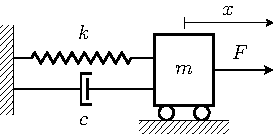
\includegraphics[width=0.4\linewidth]{000_introduction/images/Theoretical Background/Spring_Mass_Damper.pdf}
    \caption{Mass-Spring-Damper model.}
    \label{fig:mass_spring_damper}
\end{figure}

The command "htb" is here to express our priorities in the positioning of the image: h=here, t=top, b=bottom. Latex will automatically try to insert the image where it is the most "clean". However, you can override Latex' choices by replacing "htb" by "H".

For two plots in the same figure, you can use

\begin{figure}[htb]%
    \centering
    \subfloat[\centering Case A-1]{{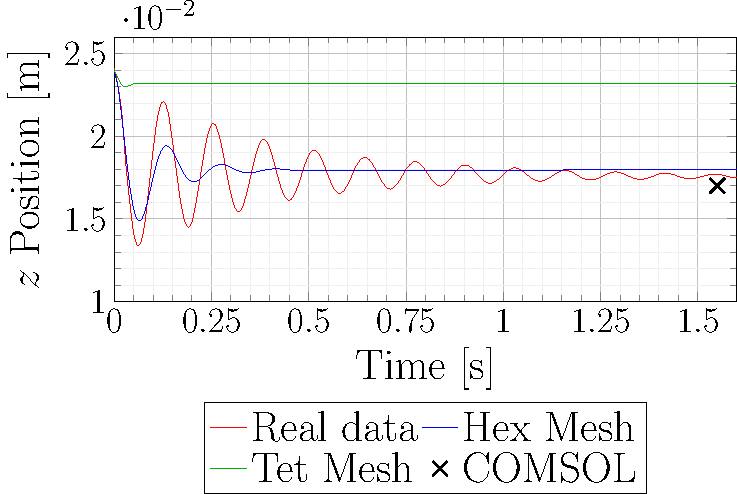
\includegraphics[width=0.42\linewidth]{000_introduction/images/Results/Gravity_Left_4608_Small.pdf}}}%
    \qquad
    \subfloat[\centering Case A-2]{{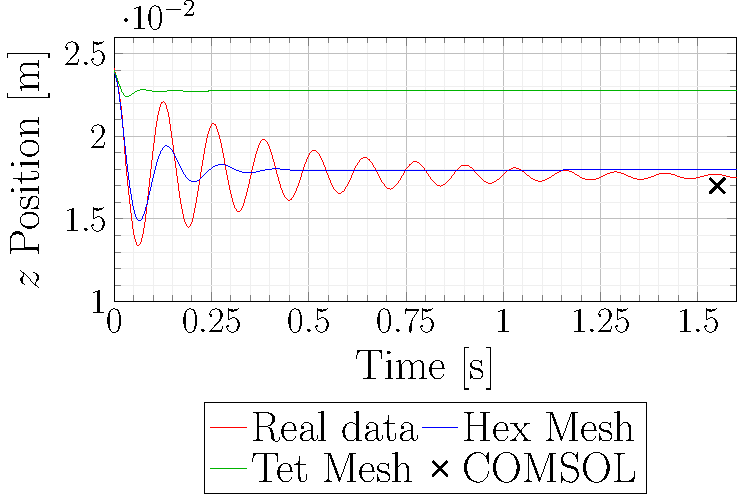
\includegraphics[width=0.42\linewidth]{000_introduction/images/Results/Gravity_Left_183516_Small.pdf}}}%
    \caption{Simulations results and comparison between the Real data, the Hex Mesh, the Tet Mesh and the COMSOL static solution.}%
    \label{fig:gravity_left}%
\end{figure}

%%%%%%%
%%%%%%% Tables
%%%%%%%
\subsection{Tables}\label{tables}

The best way to create tables is to use an online Latex table creator: \url{https://www.tablesgenerator.com/}. Here is an example:

\begin{table}[htp]
    \centering
    \begin{tabular}{@{}llllll@{}}
    \toprule
    Case & DOFs  & Type of mesh & Thread number & Time step & Average fps  \\ \midrule
    AC2  & 10416 & Hex          & 1             & 0.01      & 0.208 \\
    AC2  & 10416 & Hex          & 2             & 0.01      & 0.330 \\
    AC2  & 10416 & Hex          & 4             & 0.01      & 0.450 \\
    AC2  & 10416 & Hex          & 8             & 0.01      & 0.507 \\
    AC2  & 10416 & Hex          & 16            & 0.01      & 0.508 \\ \bottomrule
    \end{tabular}
    \caption{Influence of the number of threads on the average fps value.}
    \label{tab:thread_number}
\end{table}


%%%%%%%
%%%%%%% Equations
%%%%%%%
\subsection{Equations}\label{equations}

There are multiple ways to insert mathematical symbols or expressions in latex. For in-text you can use the dollar symbol as $\bm{q}=\bm{q}(t)\in \mathbb{R}^{3N}$. 

For equation, we suggest using the following syntax:

    \begin{equation}\label{optimization_problem}
        \min_{\bm{q}_{i+1}}\left\{ \frac{1}{2h^2}||\bm{M}^{\frac{1}{2}}(\bm{q}_{i+1}-\bm{y}_i)||_2^2 + \sum_e \frac{w_e}{2}||\bm{G_e}\bm{q}_{i+1}-\bm{z_e}^\ast (\bm{q}_{i+1})||_2^2 \right\}
    \end{equation}
    
You should label your equations, so that you can refer to them as \Cref{optimization_problem}.


%%%%%%%
%%%%%%% References
%%%%%%%
\subsection{References}\label{references}

References are taken from your ".bib" file. This document has to be include in the "main.tex" file. Every entry of the bib file has a specific name. Knowing this name, you can cite the reference using \citep{Bouaziz2014}, \citet{Bouaziz2014} or \cite{Bouaziz2014}. 
